\section{正交投影}
\label{sec:ipspace-orthogonal-projection}

章首问：在$L^2[-1,1]$中用常数近似$x^2$，哪个常数最好？更一般地，给定Hilbert空间$H$中的一个子空间$M$与一个目标$f$，能否在$M$中找到离$f$最近的元素。有限维中，卷二证明了最近点存在、唯一，并且误差与子空间正交。无限维中新的问题是：逼近距离的下确界能否被取到。本节证明，只要$H$完备、$M$闭，答案就是肯定的。

\paragraph{正交补}
先给出“与整个子空间垂直”的元素组成的集合。对子集$M\subseteq H$，令
\[
 M^\perp=\{g\in H:\ \langle m,g\rangle=0\ \text{对所有}\ m\in M\},
\]
称为$M$的\term{正交补}（orthogonal complement）。它是线性子空间，因为内积对第二个变量线性。它还是闭集：若$g_n\in M^\perp$且$g_n\to g$，由内积的连续性，$\langle m,g\rangle=\lim_n\langle m,g_n\rangle=0$对每个$m\in M$成立。所以无论$M$本身是否闭，$M^\perp$总是闭线性子空间。

\paragraph{最佳逼近的存在与唯一}
设$M\subseteq H$是线性子空间，$f\in H$，记
\[
 d=d(f,M)=\inf_{m\in M}\lVert f-m\rVert .
\]
下确界总是存在的。问题在于是否有$m\in M$恰好取到它：在无限维中，越来越好的近似可能没有极限，极限也可能离开$M$。下面的定理说明，完备性和闭性分别排除这两种情况，而平行四边形恒等式保证越来越好的近似确实彼此接近。

\begin{theorem}[闭子空间上的最佳逼近]
\label{thm:ipspace-best-approximation}
设$H$是Hilbert空间，$M\subseteq H$是闭线性子空间。则对每个$f\in H$，存在唯一的$m_*\in M$使$\lVert f-m_*\rVert=d(f,M)$。
\end{theorem}

\begin{proof}
取$m_n\in M$使$\lVert f-m_n\rVert^2<d^2+1/n$，称为极小化序列。

第一步，极小化序列是柯西列。对$f-m_j$与$f-m_k$用平行四边形恒等式~\eqref{eq:ipspace-parallelogram}，
\[
 \lVert m_j-m_k\rVert^2=2\lVert f-m_j\rVert^2+2\lVert f-m_k\rVert^2-4\Bigl\lVert f-\frac{m_j+m_k}2\Bigr\rVert^2 .
\]
$M$是线性子空间，中点$\tfrac{m_j+m_k}2$在$M$中，所以最后一项中的范数平方至少为$d^2$。于是$\lVert m_j-m_k\rVert^2<2(d^2+\tfrac1j)+2(d^2+\tfrac1k)-4d^2=\tfrac2j+\tfrac2k$，$(m_n)$是柯西列。

第二步，极限存在且留在$M$中。$H$完备，所以$m_n$收敛到某个$m_*\in H$；$M$闭，所以$m_*\in M$。由范数的连续性，$\lVert f-m_*\rVert=\lim_n\lVert f-m_n\rVert=d$。

第三步，唯一性。若$m_*,m_*'\in M$都取到$d$，则二者交替排列成的序列$m_*,m_*',m_*,m_*',\ldots$也是极小化序列，由第一步是柯西列，所以$m_*=m_*'$。
\end{proof}

三个条件各有分工。平行四边形恒等式说明：若两个点离$f$都几乎是最近的，它们彼此必然很近，这一步依赖内积，一般Banach空间中最近点可能不唯一，也可能不存在。$H$的完备性给出极小化序列的极限，$M$的闭性保证这个极限没有离开$M$。实际上前两步只用到$M$自身的完备性：若$M$在限制后的范数下完备，即使$H$不完备，结论也成立，这适用于任意内积空间中的有限维子空间。

\paragraph{误差正交与正交投影}
最近点还可以用正交关系刻画，这是计算它的实用方法。

\begin{theorem}[正交刻画]
\label{thm:ipspace-orthogonality-characterization}
设$H$是Hilbert空间，$M\subseteq H$是闭线性子空间，$f\in H$，$m_*\in M$。则$\lVert f-m_*\rVert=d(f,M)$当且仅当$f-m_*\in M^\perp$。此时对任意$m\in M$，
\begin{equation}
 \lVert f-m\rVert^2=\lVert f-m_*\rVert^2+\lVert m_*-m\rVert^2 .
 \label{eq:ipspace-pythagoras}
\end{equation}
\end{theorem}

\begin{proof}
设$m_*$取到$d$，记$r=f-m_*$。任取$m\in M$与$t\in\mathbb K$，$m_*+tm\in M$，所以$\lVert r\rVert^2\leq\lVert r-tm\rVert^2=\lVert r\rVert^2-2\operatorname{Re}\bigl(t\langle r,m\rangle\bigr)+\lvert t\rvert^2\lVert m\rVert^2$。取$t=s\,\overline{\langle r,m\rangle}$，$s>0$为实数，得$2s\lvert\langle r,m\rangle\rvert^2\leq s^2\lvert\langle r,m\rangle\rvert^2\lVert m\rVert^2$。两边除以$s$再令$s\to0$，得$\langle r,m\rangle=0$。所以$r\in M^\perp$。

反过来，设$r=f-m_*\in M^\perp$。对任意$m\in M$，$m_*-m\in M$与$r$正交，展开$\lVert r+(m_*-m)\rVert^2$时交叉项为零，得式~\eqref{eq:ipspace-pythagoras}。于是$\lVert f-m\rVert\geq\lVert f-m_*\rVert$，等号当且仅当$m=m_*$，$m_*$是最近点。
\end{proof}

式~\eqref{eq:ipspace-pythagoras}是勾股关系：$f$、$m_*$、$m$三点构成以$m_*$为直角顶点的直角三角形，见图~\ref{fig:ipspace-projection-geometry}。它不仅说明$m_*$最近，还定量地给出任何其他候选多出的误差，恰为它到$m_*$的距离平方。

\begin{figure}[!htb]
  \centering
  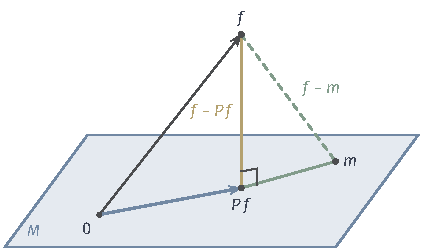
\includegraphics[width=71.7mm]{figures/02-abstract-mathematics/03-function-spaces/tikz/c1-projection-geometry/figure.pdf}
  \caption{闭子空间上的正交投影（示意）。平面代表闭子空间$M$，$Pf$是$M$中离$f$最近的点，误差$f-Pf$与$M$垂直。对$M$中任意另一点$m$，三点构成直角三角形，$\lVert f-m\rVert^2=\lVert f-Pf\rVert^2+\lVert Pf-m\rVert^2$，所以$m$离$f$更远。}
  \label{fig:ipspace-projection-geometry}
\end{figure}

\begin{definition}[正交投影]
\label{def:ipspace-orthogonal-projection}
设$M$是Hilbert空间$H$的闭线性子空间。把定理~\ref{thm:ipspace-best-approximation}中的最近点$m_*$记为$P_Mf$，称为$f$在$M$上的\term{正交投影}（orthogonal projection）。
\end{definition}

\paragraph{正交分解}
由定理~\ref{thm:ipspace-orthogonality-characterization}，每个$f\in H$都可以写成
\[
 f=P_Mf+(f-P_Mf),\qquad P_Mf\in M,\quad f-P_Mf\in M^\perp .
\]
这种分解是唯一的：若$f=m+g=m'+g'$，$m,m'\in M$，$g,g'\in M^\perp$，则$m-m'=g'-g$同时属于$M$与$M^\perp$，与自己正交，只能为零。所以$H$中每个元素唯一地分成$M$中的部分与$M^\perp$中的部分，记作$H=M\oplus M^\perp$。

由勾股关系还得到$\lVert f\rVert^2=\lVert P_Mf\rVert^2+\lVert f-P_Mf\rVert^2$，所以$\lVert P_Mf\rVert\leq\lVert f\rVert$。$P_M$的线性也可以从正交刻画读出：$af+bg-(aP_Mf+bP_Mg)$是两个$M^\perp$中元素的组合，仍在$M^\perp$中，所以$aP_Mf+bP_Mg$就是$af+bg$的投影。把$P_M$作为线性算子研究，是第~\ref{chap:linear-operators}章的内容。

\paragraph{向常数投影}
回到章首的问题。在$L^2[-1,1]$中取$M=\operatorname{span}\{1\}$，它是一维子空间，因而闭。由正交刻画，$c$是最佳常数当且仅当$\langle1,f-c\rangle=\int_{-1}^1(f-c)\,dx=0$，即
\[
 c=\frac12\int_{-1}^1f(x)\,dx ,
\]
最佳常数就是平均值。对$f=x^2$，$P_Mf=\tfrac13$，误差$x^2-\tfrac13$与$1$正交，距离平方为
\[
 \int_{-1}^1\Bigl(x^2-\frac13\Bigr)^2dx=\frac25-\frac49+\frac29=\frac8{45}.
\]
由式~\eqref{eq:ipspace-pythagoras}，任何其他常数$c$的误差平方都是$\tfrac8{45}+2(c-\tfrac13)^2$。

\paragraph{闭性不能去掉}
定理~\ref{thm:ipspace-best-approximation}中的闭性是必要的。在$\ell^2$中取$M=c_{00}$，它是线性子空间但不闭。令$f=(1,\tfrac12,\tfrac13,\ldots)\in\ell^2$。截断$x^{(N)}\in c_{00}$满足$\lVert f-x^{(N)}\rVert^2=\sum_{k>N}1/k^2\to0$，所以$d(f,c_{00})=0$。若下确界被某个$m\in c_{00}$取到，则$\lVert f-m\rVert=0$，$f=m$有无穷多项非零，矛盾。最近点不存在：每个有限支撑数列都可以再改进，却没有最好的那一个。

\paragraph{与一般闭凸集的分工}
定理~\ref{thm:ipspace-best-approximation}的第一、二步只用到两件事：中点$\tfrac{m_j+m_k}2$仍在$M$中，以及$M$闭。所以把$M$换成任意非空闭凸集$C$，同样的论证给出最近点的存在与唯一。但定理~\ref{thm:ipspace-orthogonality-characterization}用到了$m_*+tm\in M$对所有$t$成立，这是线性子空间的性质；对闭凸集，正交条件要换成变分不等式$\operatorname{Re}\langle f-m_*,c-m_*\rangle\leq0$（$c\in C$），投影也不再是线性映射。闭凸集上的投影及其在优化算法中的使用，可参考\BookChapterRef{chap:nonsmooth-composite-optimization}{卷五第4章“非光滑与复合优化”}。本章只处理线性子空间。
